\documentclass[sigconf]{acmart}

\usepackage{graphicx}
\usepackage{hyperref}
\usepackage{todonotes}

\usepackage{endfloat}
\renewcommand{\efloatseparator}{\mbox{}} % no new page between figures

\usepackage{booktabs} % For formal tables

\settopmatter{printacmref=false} % Removes citation information below abstract
\renewcommand\footnotetextcopyrightpermission[1]{} % removes footnote with conference information in first column
\pagestyle{plain} % removes running headers

\newcommand{\TODO}[1]{\todo[inline]{#1}}

\begin{document}
\title{Big Data and Artificial Intelligence with Computer Vision}

\author{Bharat Mallala}
\affiliation{%
  \institution{Indiana University}
  \city{Bloomington, IN 47408} 
  \country{USA}}
\email{bmallala@iu.edu}






% The default list of authors is too long for headers}
%\renewcommand{\shortauthors}{B. Trovato et al.}


\begin{abstract}
Big data refers to a problem of dealing with huge volumes of data. With the increase in the amount of data generated every day from various fields, it is becoming extremely hard to store and process this data efficiently. Artificial Intelligence is a research field aiming at replicating human work through machines. Computer vision refers to a research area within AI dealing with training computers to recognize certain subjects of interest. With the exponential growth of AI and computer vision in the recent years, there is need to address the big data problem associated with it.
\end{abstract}

\keywords{Artificial Intelligence, Computer vision, Perceptron Deep Learning, Convolutional Neural Networks }


\maketitle

\section{Introduction}
Artificial Intelligence is an aim at replicating human intelligence through machines. The term AI was in existence form the late 1950's during which there was a lot of enthusiasm on its potential during which Alan Turing introduced the Turing test. A lot of research was carried out in AI during the 1960's with the introduction of perceptron theory and its ability to solve problems. There was a major setback for AI in the early 1970's during which Minsky in his book on perceptrons has pointed out the major drawbacks of perceptrons in dealing with complex problems.\cite{Crandall}

There has been a consistent growth in AI from the 1990's with the introduction of the statistical approach to problem-solving. With the increase in the use of Big data from 2010, there was a lot of development in the field of AI with many voice assistants, self-driving cars, automated robots etc. Many AI problems which were np-hard previously would now take minutes to solve thanks to recent advancements in big data. Professor Crandall quoted during his lecture quoted that "Problems that seem to require intelligence usually require exploring multiple choices".\cite{Crandall}, which is a way of exhibiting intelligence without actually having it. For example for a machine to win a tic-tac-toe game against a human it basically has to explore all the possible choices, it can make from any given state.

Hence we can map an AI problem as a search problem, but it usually requires searching through huge search spaces, this is when it becomes a Big data problem. For example, for a computer t win against a human in chess it needs to search through hundreds of thousands of states. To deal with such huge data, there is a need to apply big data technologies to better store data and efficiently manage it. Ai problems typically involve using both structured and unstructured kind of data in huge volumes. The traditional RDBMS methods have a hard time dealing with unstructured data. This is an area where Big data shines with the ability to deal with both structured and unstructured data efficiently.

"Computer vision is an interdisciplinary field that deals with how computers can be made for gaining high-level understanding from digital images or videos".\cite{www-wiki1} It is an area of research within AI that aims at recognizing subjects in an environment from images or videos. Convolutional Neural Networks shines at image classification from images with minimal prepossessing of the input variables and still manages to obtain better classification. With the exponential rise of AI and especially CNN lately, there is an increased interest in computer vision for researchers. Computer vision involves training the model with huge sets of images and videos which indeed needs to be addressed using big data technologies.

\section{Rethinking the Inception Architecture for Computer Vision}

\subsection{CNN's for Computer vision}

Convolutional Neural Networks(CNN's) is the key to advancements in computer vision in the recent years with its low parameter count and computational efficacy. A CNN has multiple layers with perceptrons in them that help in the information flow from the input to output. A CNN typically has filters that are mapped across the original image to extract useful features from the image. During the training phase of the model, CNN learns the values of the filters. A CNN architecture has mainly two phases convolution phase and pooling phase. In the convolution phase features are extracted from the image using filters. In the pooling phase, the width of the feature map is reduced by applying various techniques. This is done to remove unnecessary data from the features. These stages are iterated till the desired features are obtained from the image.\cite{Williamson}   Figure 1 shows a typical CNN architecture.\cite{google}

\subsection{Design}
A lot of design principles need to be followed when designing a CNN. With the numerous number of iterations required for the CNN phases, a good design decision can vastly improve the efficiency.Avoiding bottlenecks/cycles in the CNN helps in smooth flow of information which otherwise can drastically reduce the performance of the CNN. The CNN is usually trained locally within the network. Using a high dimensional representation of the feature space help to in training the network at a relatively faster rate. Pooling/Spacial aggregation of the CNN helps to reduce the dimensions of the feature space which also helps in faster training. This is most helpful when we are dealing with big data and we have a huge set of training images. When dealing with huge CNN with huge depth and width of the network, there is a need to strike a balance among width and depth of the image. The depth of CNN is determined by the size of the filter used at each iteration of the network. Optimality can be obtained when increasing each of them in parallel for every iteration.\cite{Christian}

\subsection{Method}
Once the training set of images is obtained, the depth of the CNN should be formulated i.e. 1x1 layer of 3x3 layer etc. Now that the depth is determined, the next step is to determine the size of the filters. CNN with large filters usually tends to be expensive when it comes to computational cost. Hence the ideal approach will be to start with a reasonable filter size and gradually reduce it in every iteration. But a very small filter may not extract enough features from the image, hence it is important to reduce the filter size and also making sure enough features are extracted.\cite{Christian}

\subsection{Role of Big data}
With the exponential increase in the training sample for the CNN, the depth of the CNN would drastically increase making it not computationally feasible. Big data techniques needs to applied to CNN to meet the vast training requirements of computer vision. The training sample is stored across multiple node of the Hadoop architecture making more easily accessible. Each stage of the CNN is carried across multiple nodes making it computational feasible. Since Hadoop also supports semi and unstructured data as well, unprocessed images can also be trained with ease using CNN.\cite{Christian}

\section{Artificial Intelligence and Big Data}
\subsection{Contributions of AI}
With ever increasing data in the field of AI, researchers are outsourcing some of the AI tasks such as pattern recognition, deep learning to other parallel computing based methods. Typical AI systems with their extensive use in decision making for major businesses around the globe,  need to make decisions with a specific time limit. As formulated earlier if we map an AI problem as a search problem, searching through huge spaces in relatively less amount of time is a cumbersome task to do. For example, while playing a game of chess against a human, a computer cannot take an infinite amount of time to make the next move as it searches across all the possible states. Also, most AI applications typically deal with structured data as their input. But with the increase in the amount of data AI needs to be processed currently the approach to deal only with structured data no longer works. There is a need to apply other techniques to process the unstructured and semi-structured data and use it for training the AI models.\cite{OLeary}

\subsection{Limitations of AI algorithms}
Till date, much of the research is centered on using AI on a single machine which has its limitations when it comes to data storage and computational efficiency. Many of the existing data mining algorithms are limited when it comes to dealing with big data. Data might consist of some inconsistencies, for example missing data, incorrect data, etc. which leads to a majority of the AI algorithms to obtain a good accuracy\cite{OLeary}. 

\subsection{Mapreduce Approach}

Using MapReduce and address most of the above-stated limitations of AI algorithms. MapReduce in the recent times has been used for parallel-processing which can be quite useful for AI algorithms. With the approach of using parallel processing many of the machine learning algorithms, we can train the model to learn simultaneously from multiple machines, thereby drastically reducing the overall computational cost and time. Researchers have also developed a machine learning module on Hadoop called Mahout. Mahout is responsible to run all of the tasks that a traditional system can do but within a relatively less amount of time. This done using parallel data storage and processing feature of Hadoop.\cite{OLeary}


Typically in a Hadoop environment, any AI problem is divided into numerous subproblems depending upon the size of the cluster. The training data similarly is subdivided according to the tasks. Now, these tasks are allocated to all the data nodes. The metadata corresponding to the data nodes will be stored in the name-node. There will also be a secondary name-node in case the name-node fails. The zookeeper component is responsible to allocate tasks to data nodes. All these work together in real time to obtain parallel processing of the data. \cite{OLeary}

\subsection{Issues with AI and Big data}

AI and big data complement each other under numerous occasions. But there are a lot of issues when it comes to compatibility between AI and Big data. Firstly many of the iterative generic Machine learning algorithms are difficult to be used in the Hadoop environment. These algorithms do not come included with the Mahout module. So researchers are trying to address this issue of compatibility. Secondly, there has been an inconsistency in Data visualization part of AI. AI algorithms, when used in traditional systems, are capable of creating some great visualizations to make the results of the model more appearing. By using AI within Hadoop environment the level of visualizations supported on Hadoop is mediocre. Third, AI algorithms can be used to model real-time data and make inferences from the same. When it comes to Hadoop we have a component 'Flume', But it does not support the level of detail as the traditional systems.Fourth, Hadoop environment is not so well equipped when it comes to dealing with audio/video file which the traditional algorithms are more capable of. \cite{OLeary}

\section{Conclusion}
Artificial Intelligence with its ability to take over the world has some limitations when it comes with Big data, i.e. huge volumes and different varieties of data. With the advancements in Big data and its technologies, this gap between the two can be reasonably reduced by making modifications to existing AI approaches to make it compatible with Big data. Mahout is one of the Big data modules by which we can apply many of the AI algorithms to Big data. Advancements in Computer vision has led to extensive use of CNN's for applications such as image recognition. Big data has provided a means to apply computer vision techniques on a much larger scale with low computational cost in a relatively lesser time. 

\begin{acks}
I would like to thank Dr. Gregor von Laszewski and the AI's for all the help they have provided for this paper.

\end{acks}

\bibliographystyle{ACM-Reference-Format}
\bibliography{report} 

\begin{figure}[htp]
    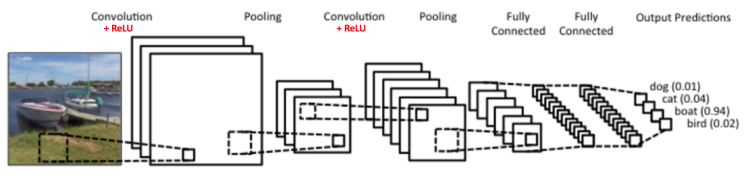
\includegraphics[width=1\textwidth]{image1.png}
    \caption{Convolutional Network Architecture \cite{google}}
    \label{fig:figure1}
\end{figure}
\end{document}
